\documentclass[10pt,letterpaper]{article}
\usepackage[latin1]{inputenc}
\usepackage{amsmath}
\usepackage{amsfonts}
\usepackage{amssymb}
\usepackage{graphicx}
\usepackage[margin=1in]{geometry}
\usepackage{listings}
\usepackage{float}
\usepackage{fancyhdr}
\pagestyle{fancy}
\lhead{\today}
\chead{Project 4}
\rhead{Tan, Zhou}
%\usepackage[margin=1in]{geometry}
\usepackage{color} %red, green, blue, yellow, cyan, magenta, black, white
\definecolor{mygreen}{RGB}{28,172,0} % color values Red, Green, Blue
\definecolor{mylilas}{RGB}{170,55,241}

\newcommand{\ssbracket}[2]{#1^{(#2)}}

\author{Hao Hui Tan(999741711, tanstev1)\\Kyle Zhou (1000959732, zhoukyle)}
\title{CSC411H1S Project 4}
\begin{document}
	\lstset{language=Python,%
		%basicstyle=\color{red},
		breaklines=true,%
		%morekeywords={matlab2tikz},
		keywordstyle=\color{blue},%
		morekeywords=[2]{1}, keywordstyle=[2]{\color{black}},
		identifierstyle=\color{black},%
		stringstyle=\color{mylilas},
		commentstyle=\color{mygreen},%
		showstringspaces=false,%without this there will be a symbol in the places where there is a space
		numbers=left,%
		numberstyle={\tiny \color{black}},% size of the numbers
		numbersep=9pt, % this defines how far the numbers are from the text
		emph=[1]{for,end,break},emphstyle=[1]\color{red}, %some words to emphasise
		%emph=[2]{word1,word2}, emphstyle=[2]{style},
		caption=\lstname,
	}

	\maketitle
	\newpage
	\begin{enumerate}
		\item %1
		The board is represented by a flat 9-element NumPy tuple.
		Turn denotes whose turn it is (1 for X, 2 for O).
		Done denotes whether the game is done (True if game is over, False otherwise.)

		Below is an example of a sample game played against myself.
		\begin{verbatim}
Python 2.7.14 |Anaconda custom (64-bit)| (default, Oct  5 2017, 02:28:52)
[GCC 4.2.1 Compatible Clang 4.0.1 (tags/RELEASE_401/final)] on darwin
env.render()
====
env.step(0)
Out[3]: (array([1, 0, 0, 0, 0, 0, 0, 0, 0]), 'valid', False)
env.render()
x..
====
env.step(4)
Out[5]: (array([1, 0, 0, 0, 2, 0, 0, 0, 0]), 'valid', False)
env.render()
x..
.o.
====
env.step(8)
Out[7]: (array([1, 0, 0, 0, 2, 0, 0, 0, 1]), 'valid', False)
env.render()
x..
.o.
..x
====
env.step(2)
Out[9]: (array([1, 0, 2, 0, 2, 0, 0, 0, 1]), 'valid', False)
env.render()
x.o
.o.
..x
====
env.step(6)
Out[11]: (array([1, 0, 2, 0, 2, 0, 1, 0, 1]), 'valid', False)
env.render()
x.o
.o.
x.x
====
env.step(3)
Out[13]: (array([1, 0, 2, 2, 2, 0, 1, 0, 1]), 'valid', False)
env.render()
x.o
oo.
x.x
====
env.step(7)
Out[15]: (array([1, 0, 2, 2, 2, 0, 1, 1, 1]), 'win', True)
env.render()
x.o
oo.
xxx
====
env.done
Out[17]: True
env.step(1)
Out[18]: (array([1, 0, 2, 2, 2, 0, 1, 1, 1]), 'done', True)
		\end{verbatim}
		\item %2
		\begin{enumerate}
			\item %2a
			The following is the new implemented policy
\begin{lstlisting}
class Policy(nn.Module):
    """
    The Tic-Tac-Toe Policy
    """
    def __init__(self, input_size=27, hidden_size=64, output_size=9):
        super(Policy, self).__init__()

        self.linear1 = nn.Linear(input_size, hidden_size)
        self.linear2 = nn.Linear(hidden_size, output_size)

    def forward(self, x):
        x = F.relu(self.linear1(x))
        x = self.linear2(x)
        return F.log_softmax(x)
\end{lstlisting}
			\item %2b
			The 27 dimensions are a flattened encoding of a one-hot encoding of the state of the board.
			If \verb|.view(3,9)| is applied to the array, the columns would be the one-hot encoding of each cell in the board (starting from the top left, going across each row, and ending in the bottom right).

			If a column contains ``1 0 0,'' the cell is empty.\\
			If a column contains ``0 1 0,'' the cell is occupied by an X.\\
			If a column contains ``0 0 1,'' the cell is occupied by an O.
			%The function first creates a one-hot encoding of the state at each cell of the board, flattens it, then passes it into the Policy neural network.
			%The function then samples a state from the output of the network, and calculates the loss function (in this case, log probability).
			%The function then returns the chosen move (i.e. chosen next state) with its corresponding loss value.
			\item %2c
			The value in each dimension means the chance that making the move (e.g. adding an X into that cell) would result in winning the game.
			This policy is stochastic because it samples the next move from a distribution, rather than following a deterministic algorithm.
		\end{enumerate}
		\item %3
		\begin{enumerate}
			\item %3a
			The implementation of \textbf{compute\_returns} is shown below.
			\begin{lstlisting}
def compute_returns(rewards, gamma=1.0):
    """
    Compute returns for each time step, given the rewards
      @param rewards: list of floats, where rewards[t] is the reward
                      obtained at time step t
      @param gamma: the discount factor
      @returns list of floats representing the episode's returns
          G_t = r_t + \gamma r_{t+1} + \gamma^2 r_{t+2} + ...

    >>> compute_returns([0,0,0,1], 1.0)
    [1.0, 1.0, 1.0, 1.0]
    >>> compute_returns([0,0,0,1], 0.9)
    [0.7290000000000001, 0.81, 0.9, 1.0]
    >>> compute_returns([0,-0.5,5,0.5,-10], 0.9)
    [-2.5965000000000003, -2.8850000000000002, -2.6500000000000004, -8.5, -10.0]
    """
    # TODO
    result = []
    for index in range(len(rewards)):
        sum_returns = 0
        power = 0
        for i in range(index, len(rewards)):
            sum_returns = sum_returns + ((gamma ** power) * rewards[i])
            power = power + 1
        result.append(sum_returns)
    return result
			\end{lstlisting}
			\item %3b
			If we update the weights in the middle of an episode, it would lead to erroneous results since the algorithm does not know the terminal state of the episode when it's updating the weights. For instance, if the terminal state for an agent is "loss", then this will cancel out all the rewards that are associating with the agent's previous actions in the episode. Therefore, we should not update the weights in the middle of an episode.
		\end{enumerate}
		\item %4
		\begin{enumerate}
			\item %4a
			\begin{lstlisting}
def get_reward(status):
    """Returns a numeric given an environment status."""
    return {
        Environment.STATUS_VALID_MOVE  : 0,
        Environment.STATUS_INVALID_MOVE: -99,
        Environment.STATUS_WIN         : 1,
        Environment.STATUS_TIE         : 0,
        Environment.STATUS_LOSE        : -1
    }[status]
			\end{lstlisting}
			\item %4b
			%Explain the choices that you made in 4(a). Are there positive rewards? Negative rewards? Zero rewards? Why? Explain how you chose the magnitude of the positive and negative rewards.
			The reward for a valid move is $0$, since a single valid move doesn't directly contribute to a win or a loss.
			The reward for an invalid move is $-99$, since we really don't want our neural network to try invalid moves.
			Making invalid moves is worse than losing the game.
			The reward for a win is $2$, and that's because we want to encourage our neural network to optimize for wins.
			The reward for a tie is $1$, and that is because we want to encourage the neural network to finish the game, but we don't want the neural network to choose this option over a win.
			The reward for a loss is $-1$, since we want to discourage losses.
			The magnitude of these rewards are mostly close to zero, except for invalid moves.
			This is because all of the regular states are states that could occur in regular play, and since we really want to discourage invalid moves, having the rest of the rewards close together makes the $-99$ penalty more meaningful.
		\end{enumerate}
		\item %5
		\begin{enumerate}
			\item %5a
			The hyperparameter we tweaked was the  $\gamma$ value (discount factor) in order to improve the performance of the model, since a lower $\gamma$ value would help the model prioritize shorter paths to win, which is a strong strategy when it comes to playing tic tac toe.
			Longer strategies would give the opponent more of an opportunity to disrupt the strategy, or even win in the shorter term before the strategy can complete.
			\\
			The learning curve given the above rewards and the tweaked $\gamma$ value is in Figure \ref{fig:part5alearningcurve}
			\begin{figure}[H]
				\centering
				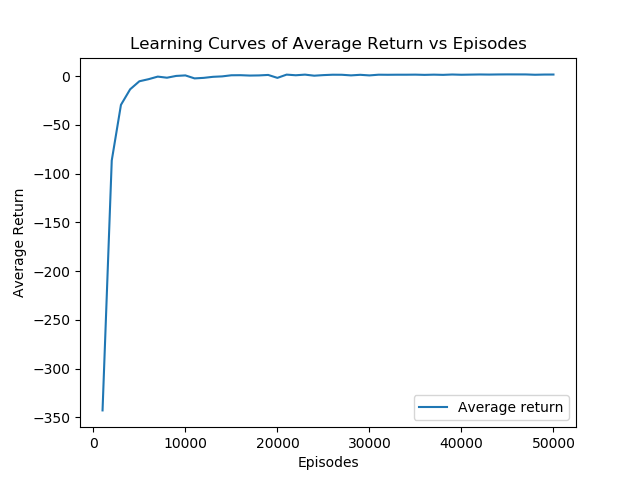
\includegraphics[width=0.7\linewidth]{Part5aLearningCurve}
				\caption{Initial Learning Curve}
				\label{fig:part5alearningcurve}
			\end{figure}

			\item %5b
			I have tuned the hyper-parameter number of hidden units by the following 3 values: 128, 32, 80. I have used the average return value at the last episode for performance metrics because this value reflects how well the trained model performs when it is being used to play against AI or human players. The learning curves of the 3 tests are shown below. \textbf{Note:} We have commented out the function call \textbf{part5b()} in the main function of the code. To reproduce the graphs and the stats below, please uncomment the line that says \textbf{part5b()}

			\begin{figure}[H]
				\centering
				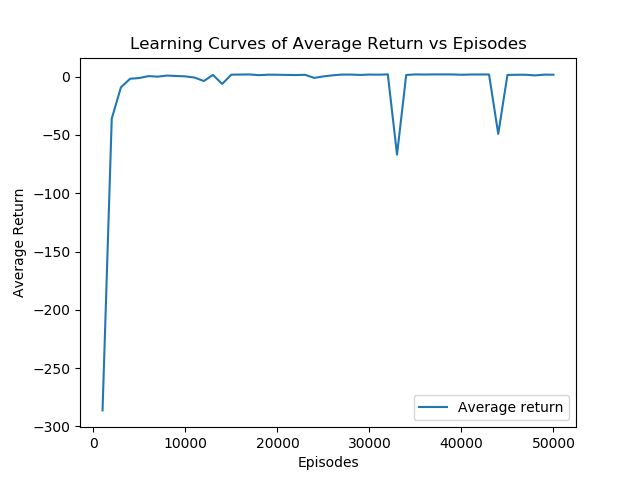
\includegraphics[width=0.7\linewidth]{Part5BLearningCurve_128.png}
				\caption{Learning Curve with 128 hidden units}
				\label{fig:part5b_128}
			\end{figure}

			\begin{figure}[H]
				\centering
				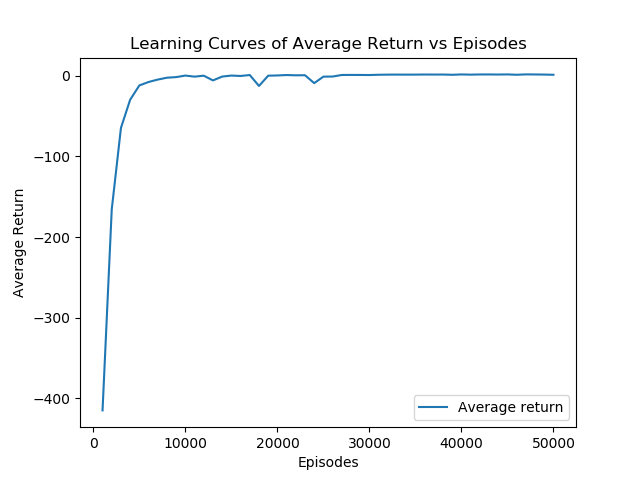
\includegraphics[width=0.7\linewidth]{Part5BLearningCurve_32.png}
				\caption{Learning Curve with 32 hidden units}
				\label{fig:part5b_32}
			\end{figure}

			\begin{figure}[H]
				\centering
				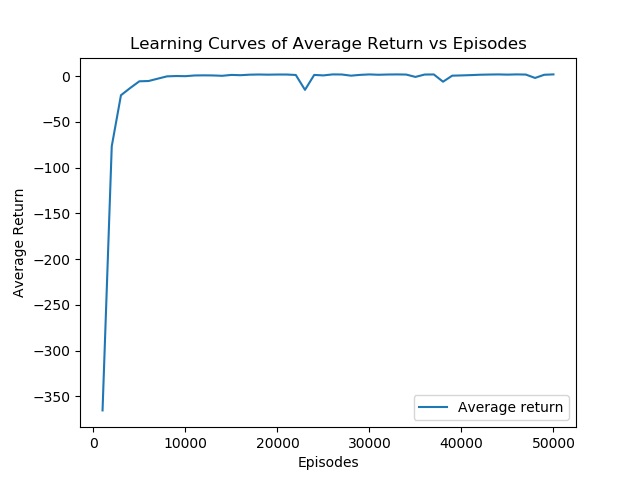
\includegraphics[width=0.7\linewidth]{Part5BLearningCurve_80.png}
				\caption{Learning Curve with 80 hidden units}
				\label{fig:part5b_80}
			\end{figure}

			The average return values for the 3 tests are as follows: \newline

			\textbf{128 Hidden Units}: 1.62          \newline
			\textbf{32 Hidden Units}: 1.41           \newline
			\textbf{80 Hidden Units}: 1.91           \newline

			From testing, the algorithm with 80 hidden units has the best performance.
			\item %5c
			The policy learned to stop playing invalid moves between 13000 and 14000 episodes.
			This was determined by recording the number of invalid moves during training, and aggregating them into 1000-episode chunks.
			When the average number of invalid moves per episode falls below 30\% (30 per 1000), that's when we know the policy has learned to stop playing invalid moves.
			% TODO include a graph
			\item %5d
		\end{enumerate}
		\item %6
		The graph that illustrates the win/lose/tie rates is shown below:

		\begin{figure}[H]
				\centering
				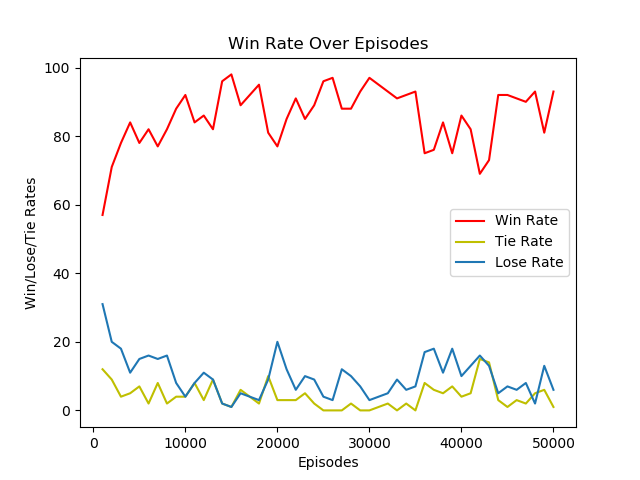
\includegraphics[width=0.7\linewidth]{Part6LearningCurve.png}
				\caption{Win Rate Over the Episodes}
				\label{fig:part6}
		\end{figure}

		From the figure above we can see the win rate generally goes up when the number of episodes increases and the lose/tie rate goes down. The result above shows the reward/punishment numbers that we come up with earlier in part 4 are reasonable and effective as the win rate is near $90\%$ at the end.

		\item %7
		\item %8
	\end{enumerate}
\end{document}
